\documentclass[a4paper, 12pt]{report}
\usepackage{monapack}
\usepackage{hyperref}
\usepackage{indentfirst}
\usepackage{subcaption}
\graphicspath{{images/}}

\usepackage[outputdir=../auxil]{minted}
\usemintedstyle{friendly}

\student{Richard Kropáček}
\trida{B4.I}
\obor{18-20-M/01 Informační technologie}
\bydliste{Mírová 429, 385 01 Vimperk}
\datumNarozeni{11. 11. 2001}
\vedouci{Mgr. Milan Janoušek}
\nazevPrace{Správa povinných prací}
\cisloPrace{1}
\skolniRok{2020/2021}
\reditel{Ing. Jiří Uhlík}

\begin{document}

	\titulniStrana
	
	\anotace Maturitní práce se zaměřuje na návrh a realizaci webové aplikace, která má na starosti správu povinných prací odevzdaných žáky. Vyučující má možnost vytvořit zadání a případně ho upravit, nebo odstranit. Žáci mají možnost procházet jak aktuální práce, tak práce, které již odevzdali například v minulých ročnících. \\
	\textbf{Klíčová slova: } C\#; ASP.NET Core; Entity Framework Core; HTML; JavaScript; CSS; Bootstrap; MySQL; WebApp

	\annotation The graduation thesis focuses on the design and implementation of a web application, which is in charge of managing the compulsory work submitted by students. The teacher has the opportunity to create an assignment and possibly modify or delete it. Pupils have the opportunity to go through both current work and work that they have already submitted, for example, in previous years.\\
	\textbf{Keywords: } C\#; ASP.NET Core; Entity Framework Core; HTML; JavaScript; CSS; Bootstrap; MySQL; WebApp

	\licencniSmlouva{18. 04. 2021}

	\podekovani Tímto bych chtěl poděkovat Mgr. Milanu Janouškovi za vedení mé Maturitní práce, cenné rady a odborný dohled. Děkuji také za pomoc všem, kteří se jakkoliv podíleli na realizaci této práce.
	
	\obsah

	\chapter{Úvod}
    Výsledkem této maturitní práce by měla být plně funkční webová aplikace, která by umožňovala efektivní správu povinných prací, které studenti odevzdávají za všechny roky studia.\par
	Pro realizaci jsem se rozhodl využít otevřený framework pro tvorbu webových aplikací APS.NET Core vyvinutý společností Microsoft Corporation. Pro tento framework jsem se rozhodl hlavně díky jeho jednoduché implementaci, možnosti ho vyvíjet a spouštět na~platformách Windows, Linux i macOS a vysokému výkonu.\par
	Pro návrh stránky využiji architektonický vzor MVC, ten mi pomůže oddělit logiku webové aplikace (Backend) od výstupu (Frontend). Pro to, aby tento vzor byl účinný, musím si rozvrhnout oprávnění, tedy role, které se ve webové aplikaci budou vyskytovat.\par
	Mimo jiné musím vyřešit způsob registrování a následného přihlašování uživatelů, tak~aby se eliminovala možnost neoprávněného přihlášení. To vše ale nebude správně fungovat, pokud nebudu mít připravenou databázi. Tu mám v plánu vytvořit v MySQL, což je velice rozšířený otevřený systém řízení báze dat.\par
	A toto všechno je potřeba vložit do uživatelsky přívětivého rozhraní, které bude jednoduché na správu a zároveň přehledné a profesionální. S tímto mi pomůže Bootstrap 4, což je front-endový open-source určený pro návrh responzivních webů.

	\chapter{Teoretický úvod}

	\section{Programovací jazyk C\#}
	C\# je moderní, vysokoúrovňový objektově orientovaný programocí jazyk vyvinutý společností Microsoft. Jazyk C\# se řadí mezi typově bezpečné programovací jazyky. To~znamená, že nedovoluje provádět operace, které mohou véct k chybám. Tento jazyk umožnuje vývojářům vytvářet mnoho druhů zabezpečených a robusních aplikací, které běži na~platformě .NET\footnote{Vývojářská platforma pro vytváření webových, mobilních,desktopových, herních, IoT a dalších aplikací. Je podporovaná v systémech Windows, Linux a macOS.}.\par
	C\# je zároveň objektově orientovaný programovací jazyk orientovaný na součásti\footnote{Component-oriented programming language}. Z~toho vyplývá, že se zaměřuje na vytváření komponent, které jsou tvořeny často se opakujícími částmi kódu. C\# také poskytuje jazykové kontrukce pro přímou podporu těchto konceptů, což z něj dělá přirozený jazyk pro tvorbu a používání těchto softwarových komponent.\cite{CSharp}\par
		Právě pomocí tohoto jazyka se tvoří backend, tedy celá logika webové aplikace založené na APS.NET Core.
	\section{Razor}
	Razor je syntaxe pro ASP.NET používaná pro tvorbu dynamických webových stránek společně s programovacím jazykem C\#. Pomocí Razor syntaxe lze vložit do webové stránky blok kódu, který se provede na straně serveru. Soubory využíající tuto syntaxi mají příponu .cshtml.\par
	Razor syntaxe se skládá z Razor značek, C\# a HTML. Výchozím Razor jazykem je HTML. Pro označení C\# kódu využijeme symbolem @. Tímto dojde k přechodu z formátu HTML do C\#. Razor vyhodnotí výrazy jazyka C\# a vykresluje je ve výstupu HTML. Kód HTML v souborech s příponou .cshtml se vykreslí serverem beze změny.\cite{Razor}

	\section{ASP.NET, ASP.NET CORE}
	\begin{figure}[h!]
		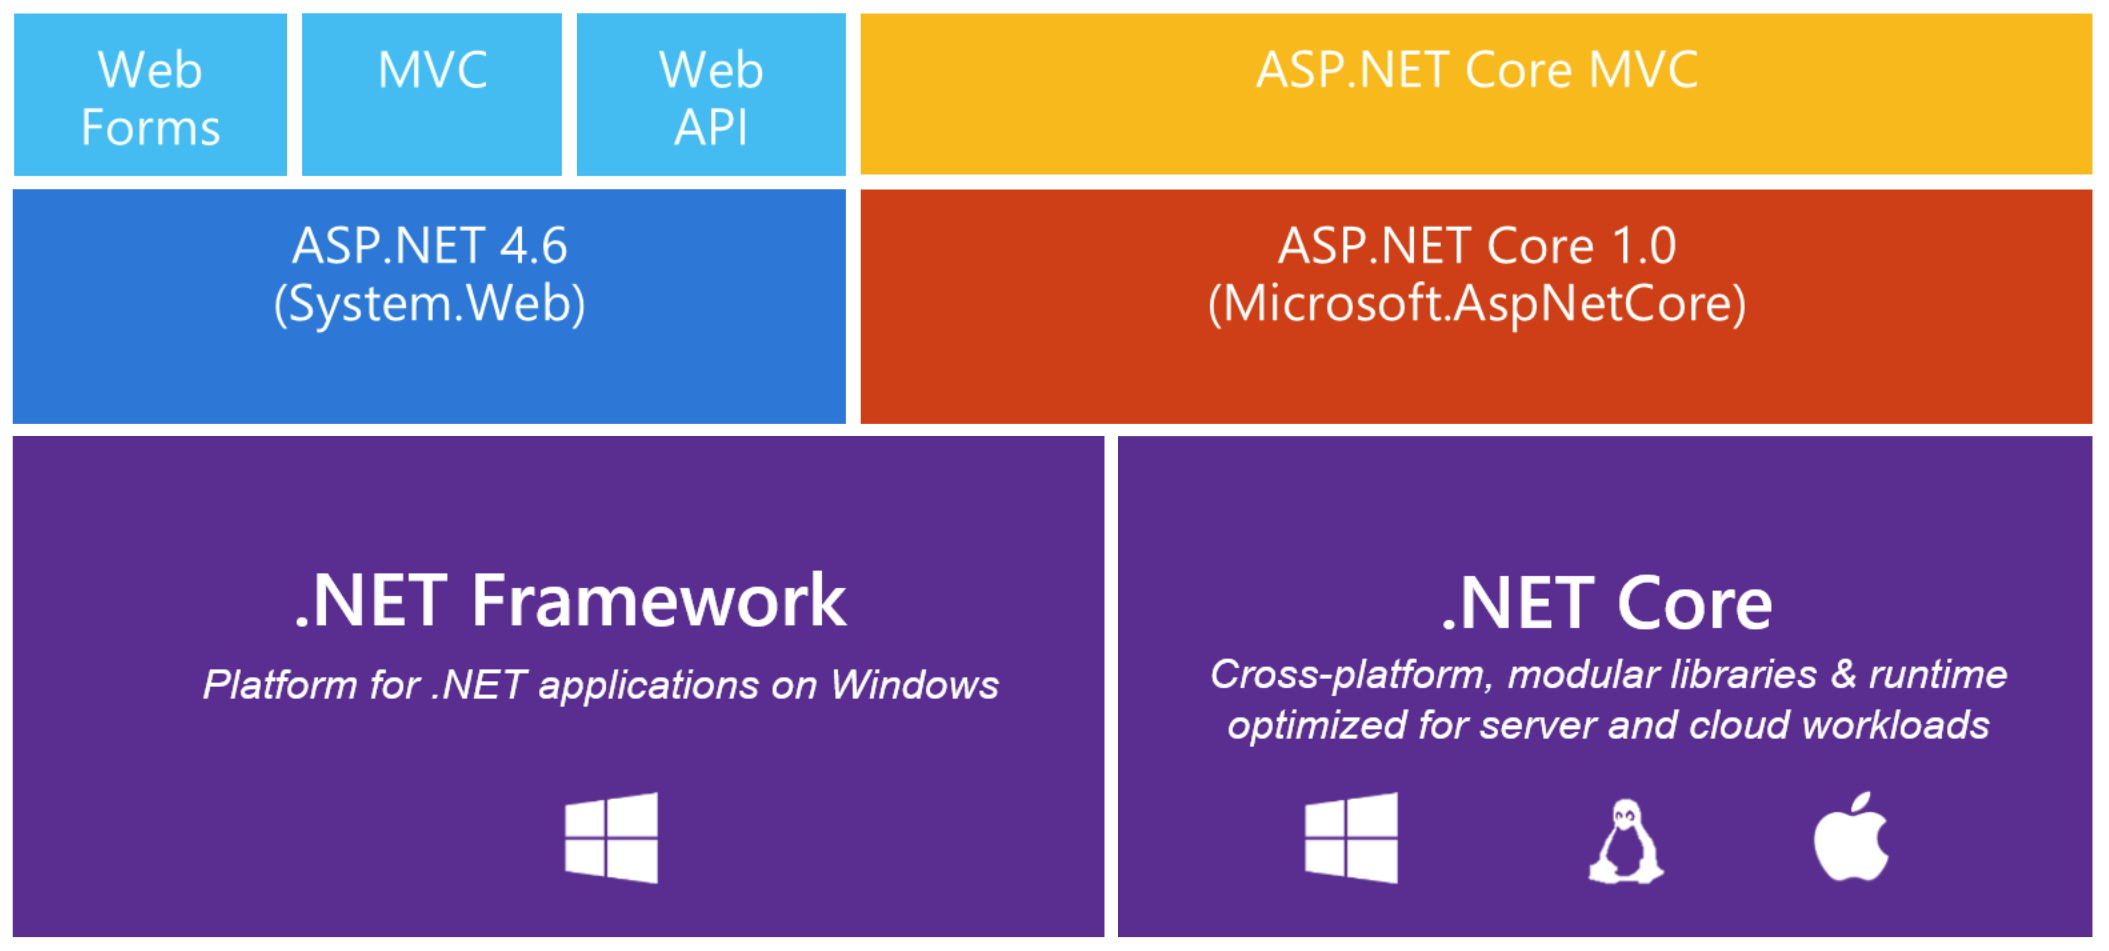
\includegraphics[width=\textwidth]{aspnetcore_aspnet}
		\caption{Porovnání ASP.NET Core a ASP.NET \cite{ASPNETCORE_ASPNET}}
		\label{ASP.NET Core a ASP.NET}
	\end{figure}
	ASP.NET je webový framework obsahující sadu knihoven, které obsahují hotová řešení mnoha základních problémů, které ve webových technologiích vyvstávají. Může se jednat např. o bezpečnost, autentifikaci uživatele, práci s databázemi apod.\par
	Tato technologie je založena na architektuře klient-server. Výstupem ASP.NET aplikace je HTML stránka. ASP.NET tedy běží na serveru a reaguje na dotazy uživatele/klienta. Pro tvorbu ASP.NET aplikace je potřeba znalost především programovacího jazyku C\# a značkovacího jazyku HTML.\cite{ASP.NET_Lekce1}

	\subsection{ASP.NET}
    ASP.NET je webový framework s otevřeným zdrojovým kódem, vytvořený společností Microsoft, pro vytváření moderních webových aplikací. ASP.NET rozšiřuje platformu .NET o nástroje a knihovny určené právě pro vytváření webových aplikací.\cite{ASP.NET}

	\subsection{ASP.NET Core}
    ASP.NET Core je open-source a multiplatformní verze ASP.NET. Tato platforma je navržena tak, aby umožnila rychlé vyvíjení runtime komponent, API, překladačů apod. a~zároveň poskytovala stabilní a podporovanou platformu pro udržení běhu aplikací.\par
	Aplikace v ASP.NET Core lze, oproti dřívější verzi APS.NET Windows-only version, vyvíjet a spouštět v systémech Windows, Linux, macOS a Docker.\cite{ASP.NET_Core}

	\section{EF6 a EF Core}
    Entity Framework je Object–relational mapping (ORM)\footnote{Objektově-relační mapování}. To znamená, že se databázové tabulky přímo mapují na C\# třídy. V projektu následně pracujeme pouze s objekty a~framework za nás na pozadí generuje SQL dotazy. Díky tomu je výsledná aplikace tvořena především pomocí objektů.\cite{ASP.NET_Lekce8}

	\subsection{Entity Framework 6}
	Entity Framework 6 (EF6) je ORM, primárně navržený pro .NET Framework, ale~zároveň s podporou pro .NET Core. EF6 je stabilní, podporovaný produkt, ale již se aktivně nevyvíjí.\cite{EF6_EFCore}

	\subsection{Entity Framework Core}
	Entity Framework Core (EF Core) je moderní ORM pro .NET. Podporuje dotazy LINQ, sledování změn, aktualizace a migrace schématu.\par EF Core pracuje s SQL Server/SQL Azure, SQLite, Azure Cosmos DB, MySQL, PostgreSQL a mnoha dalšími druhy databází.\cite{EF6_EFCore}

	\section{MVC}
	Model-View-Controller (MVC) je návrhový vzor používaný k rozdělení webové aplikace na 3 komponenty.
	\begin{itemize}
		\item Model - Práce s daty
		\item View - Uživatelské rozhraní
		\item Controller - Logická část aplikace
	\end{itemize}\par
	Pomocí vzoru MVC pro webové aplikace jsou požadavky směrovány na controller, který je zodpovědný za práci s modelem. Model provádí akce a načítá data za databáze. Controller poté zvolí zobrazení (view), které se má zobrazit, a poskytne mu model. View už pouze vykreslí stránku na základě dat získaných z modelu.\cite{MVC}

	\subsection{Model} \label{Model_teorie}
	Jedná se o dynamickou datovou strukturu aplikace, nezávislou na uživatelském rozhraní. Jejím úkolem je spravovat data, pravida a logiku aplikace. \par
	V ASP.NET Core MVC má model podobu třídy, kde veřejné metody představují položky v databázi, s kterou je třída provázaná. Ukládáme ji do adresáře Models v rámci projektu. Pomocí atributů definuje pravidla, která se aplikují na klienta a server.\cite{MVC_Wiki_EN}

	\subsection{View}
	Převádí data reprezentovaná objekty modelu do podoby vhodné k interaktivní prezentaci uživateli.\cite{MVC_Wiki_CZ} Může se jednat o jakoukoliv reprezentaci dat (graf, diagram, tabulka, atd.).\par
	V ASP.NET Core se využívá syntaxe Razor. Ta poskytuje jednoduchý, čistý a lehký způsob vykreslení obsahu HTML stránek na základě view. Razor umožňuje vykreslit stránku pomocí C\# a vytvářet webové stránky plně kompatibilní s HTML5.\cite{MVC_Wiki_EN}\par
	Každý controller může pro jedno view generovat vlastní obraz. Aby tedy nedocházelo ke kolizi 2 controlleru pro jedno view, vyžaduje  MVC uložení view do adresáře Views v rámci projektu, a zde do podadresáře s názvem controlleru, který ho generuje (\viz{ViewsController}).
	\begin{figure}[H]
		\centering
		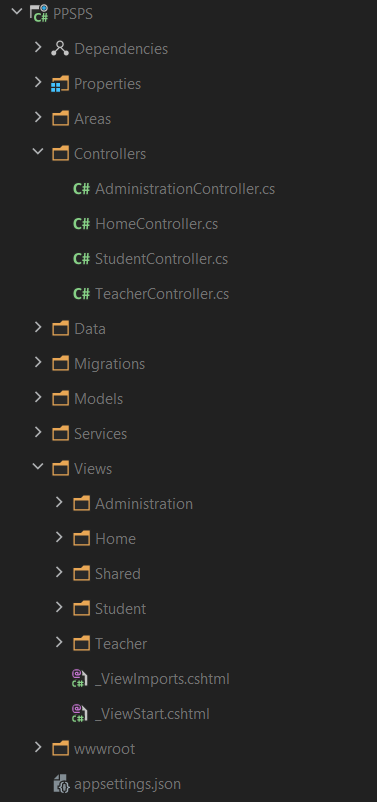
\includegraphics[scale=0.7]{ViewsController}
		\caption{Ukládání View v rámci projektu}
		\label{ViewsController}
	\end{figure}

	\subsection{Controller} \label{Controller_teorie}
	Controller reaguje na vstup uživatele a provádí interakce s objekty datového modelu. Zjednodušeně to znamená, že řadič přijme vstup, ověří jej a následně ho předá modelu.\cite{MVC_Wiki_EN}\par
	Třída controlleru obsahuje veřejné metody označené jako Action method. V ASP.NET MVC musí každý název třídy controlleru končit klíčovým slovem "Controller". To znamená, že pro domovské stránky třídu nazýváme HomeController, pro stránky studenta StudentController, apod. Všechny tyto třídy ukládáme v rámci projektu do složky Controllers.
	\begin{listing}[H]
		\inputminted{csharp}{SourceCode/Controllers/ActionMethod.cs}
		\caption{Controller - Action Method}
		\label{ActionMethod}
	\end{listing}

	\section{MySQL}
	MySQL je otevřený systém řízení báze dat uplatňující relační databázový model. Jedná se o multiplatformní databázi. Komunikace s databází probíhá pomocí dotazovacího jazyka SQL.\cite{MySQL_Wiki_CZ}\par
	Právě díky těmto vlastnostem jsem se rozhodl využít MySQL jako databázi pro tuto webovou aplikaci.

	\chapter{Základní struktura ASP.NET Core}
	Pro tuto webovou aplikaci jsem použil verzi .NET Core 3.1, ta byla vydaná v prosinci roku 2019. V době, kdy jsem začínal pracovat na tomto projektu to také byla nejnovější verze.\par
	V tomto projektu jsem dále použil ASP.NET Core Identity\footnote{Rozhraní API, které podporuje funkce přihlášení uživatelského rozhraní (UI). Spravuje uživatele, hesla, data profilu, role, deklarace identity, tokeny, potvrzení e-mailu a další.\cite{ASP.NET_Core_Identity}}, které za mě vygenerovalo základní strukturu, se kterou jsem dále pracoval.\par
	V poslední řadě bylo zapotřebí stáhnout přes NuGet package manager\footnote{NuGet je správce balíčků, který vývojářům umožňuje sdílet opakovaně použitelný kód.} Entity Framework Core a k němu nástroje potřebné k práci s MySQL databází, kterou v projektu využívám.

	\section{Model}
	Jak již bylo zmíněno v teorii (viz kapitola \ref{Model_teorie}\nameref{Model_teorie}), model se zabývá především prací s daty uloženými v~databázi. Pro to, abych s nimi mohl efektivně pracovat, potřebuji vytvořit z jednotlivých položek databáze objekty. Všechny objekty musí být veřejné, tedy public. \par
	Pro každou tabulku z databáze jsem si tedy vytvořil objekt (třídu) ve složce \textbf{Models} (\viz{ModelsFolder}). Poté jsem si potřeboval nadefinovat každou její položku jako vlastnost tohoto objetku, kde datový typ reprezentuje způsob zápisu do databáze tzn.
	\begin{itemize}
		\item VARCHAR() - Public string NazevObjektu \{ get; set; \}
		\item INT - Public int NazevObjektu \{ get; set; \}
		\item DATETIME - public DateTime NazevObjektu \{ get; set; \}
	\end{itemize}\par
	Dalším krokem bylo přiřazení atributů k jednotlivým vlastnostem. V ASP.NET Core se můžeme setkat jak s atributy, které definují vlastnosti (jedná se o primární klíč, název, formát, ...), např.
	\begin{itemize}
		\item Key - Označuje vlastnost jako primární klíč.
		\item Display("Název") - Název vlastnosti, která se zobrazí ve View.
		\item DisplayFormat(DataFormatString = "{0: yyyy-MM-dd}", ApplyFormatInEditModel = true) - Nastavuje formát zobrazení pro hodnotu vlastnosti.
	\end{itemize}
	Tak i s tzv. Atributy ověřování. Tyto atributy nám umožňují zadat pravidla pro vlastnosti objetku. V ASP.NET Core existuje několik předdefinovaných atributů, např.
	\begin{itemize}
		\item EmailAddress - Ověřuje, zda má vlastnost formát e-mailu.
		\item Range - Ověřuje, že hodnota vlastnosti spadá do zadaného rozsahu.
		\item Required - Ověří, že pole nemá hodnotu null.
		\item StringLength - Ověří, že hodnota vlastnosti řetězce nepřekračuje zadané omezení délky.
	\end{itemize}
	Atributy ověření umožňují vypsání chybové zprávy, která se zobrazí, pokud je zadán neplatný vstup do hodnoty vlastnosti. Tyto atributy je možné ověřit jak na straně klienta, tak na straně serveru.\par
	K vytvoření modelu byla nutna již navržená databáze, tu popisuji v kapitole \ref{Databaze}\nameref{Databaze} níže. Pro lepší představu přikládám zdrojový kód PPSPSSubject.cs, modelu popisující tabulku předmětů (viz zdrojový kód \ref{SubjectModel}).
	\begin{figure}[H]
		\centering
		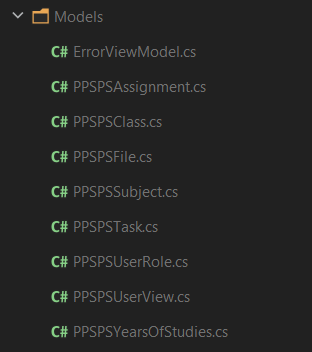
\includegraphics[scale=0.6]{Models}
		\caption{Složka Models}
		\label{ModelsFolder}
	\end{figure}
	\begin{listing}[H]
		\inputminted{csharp}{SourceCode/Models/Model.cs}
		\caption{Model - Předmět}
		\label{SubjectModel}
	\end{listing}

	\section{View}
	View lze v ASP.NET Core MVC chápat, jako HTML šablonu, do které pomocí Razor elementů vkládáme data. Pro každý controller je ve složce \textbf{Views} vytvořen vlastní adresář s názvem controlleru \viz{ViewsDetail}. V každém z těchto adresářů je poté uloženo view ve~formátu .cshtml.\par
	Ve Views adresáři je umístěn mimo jiné podadresář Shared. V něm se ukládají view, které jsou sdílené v rámci všech controllerů. Nachází se v něm většinou Layout, Partial view\footnote{Částečný pohled; Snižuje množství duplicitních kódů správou opakovaně používaných částí pohledů.}, nebo stránky s chybovým hlášením.\par
	V tomto projektu jsem si vytvořil 2 partial view. První je určený pro menu (viz kapitola \nameref{MenuPartial}) a druhý pro lištu, kde zobrazuje email přihlášeného uživatele a možnost se odhlásit (viz kapitola \nameref{LoginPartial}).\par
	Pro to, abych mohl k těmto partial přistupovat, musím do \_Layout.cshtml dopsat kód, pomoci kterého je volám, viz \ref{menupartial} pro menu a viz \ref{loginpartial} pro zobrazení emailu na liště, a~to~v~místě, kde je chci zobrazit.
	\begin{figure}[H]
		\centering
		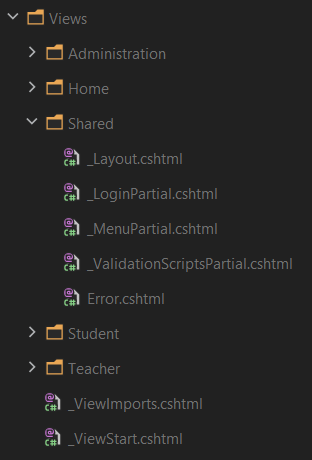
\includegraphics[scale=0.7]{ViewsDetail}
		\caption{Složka Views}
		\label{ViewsDetail}
	\end{figure}

	\subsection{\_Layout}
	V záhlaví a zápatí html souborů se nachází metadata a odkazy na CSS/Javascript. Pro to, abych nemusel zápatí a záhlaví psát do každého view, můžu je napsat právě do~souboru \_Layout.cshtml. Když se následně generuje stránka pro uživatele, načte se prvně \_Layout.cshtml a k němu se na místě, kde je volána funkce RenderBody() (viz zdrojový kód \ref{renderbody}) doplní view, které uživatel požaduje.\par
	Podobně se pracuje i s partial. Pro jejich zavolání je potřeba napsat tag <partial /> s~parametrem name, jehož hodnota je název požadovaného partial (viz zdrojové kódy \ref{loginpartial} pro~\_LoginPartial.cshtml a \ref{menupartial} pro \_MenuPartial.cshtml). Opět se volají z místa, ve kterém je chceme zobrazit.
	\begin{listing}[H]
		\inputminted{html}{SourceCode/Views/Body.html}
		\caption{View - RenderBody()}
		\label{renderbody}
	\end{listing}
	\begin{listing}[H]
		\inputminted{html}{SourceCode/Views/LoginPartial.html}
		\caption{View - Volání \_LoginPartial.cshtml}
		\label{loginpartial}
	\end{listing}
	\begin{listing}[H]
		\inputminted{html}{SourceCode/Views/MenuPartial.html}
		\caption{View - Volání \_MenuPartial.cshtml}
		\label{menupartial}
	\end{listing}

	\subsection{\_LoginPartial} \label{LoginPartial}
	Hlavník úkolem tohoto partial je zobrazit jméno uživatele, pokud je přihlášen a nabídnout mu možnost se odhlásit (\viz{ListaPrihlaseny}). Prvním krokem je, pomocí podmínky zjistíme, zda je uživatel přihlášen (SignInManager.IsSignedIn(User)). Pokud není, podmínka není splněna a partial se nezobrazí. Pokud ale je, požádá se o uživatelské jméno přihlášeného uživatele (email) a to se následně zobrazí s tlačítkem pro odhlášení (viz zdrojový kód \ref{sharedloginpartial}).
	\begin{figure}[h!]
		
\includegraphics[width=\textwidth]{ListaPrihlaseny}
		\caption{Lišta s uživatelským jménem a tlačítkem odhlášení.}
		\label{ListaPrihlaseny}
	\end{figure}
	\begin{listing}[H]
		\inputminted{html}{SourceCode/Views/Shared/_LoginPartial.html}
		\caption{View - \_LoginPartial.cshtml}
		\label{sharedloginpartial}
	\end{listing}

	\subsection{\_MenuPartial} \label{MenuPartial}
	Dalším úkolem bylo zobrazení menu (\viz{Menu}). Jako v předešlém případě ověříme, zda je uživatel přihlášen pomocí podmínky (SignInManager.IsSignedIn(User)). Pokud je uživatel přihlášen, zjišťuje se, jako má roli. Přikládám jako příklad část zdrojového kódu \ref{sharedmenupartial}, kde ověřuji, zda je uživatel ověřený (User.Identity.IsAuthenticated)\footnote{Pokud je uživatel přihlášený pomocí uživatelského jména a hesla, je i ověřený.}, a pokud ano, zda má uživatel roli Administrator (User.IsInRole("Administrator")). V tomto případě můžou nastat 3 situace:
	\begin{enumerate}
			\item Pokud je uživatel přihlášen a má roli administrátora, zobrazí se mu menu se všemi položkami.
			\item Pokud je uživatel přihlášen ale nemá roli administrátora, zobrazí se mu menu pouze s položkou Domovská stránka.
			\item Pokud není uživatel přihlášen, nezobrazí se mu menu vůbec.
	\end{enumerate}\par
	\begin{figure}[h!]
		\centering
		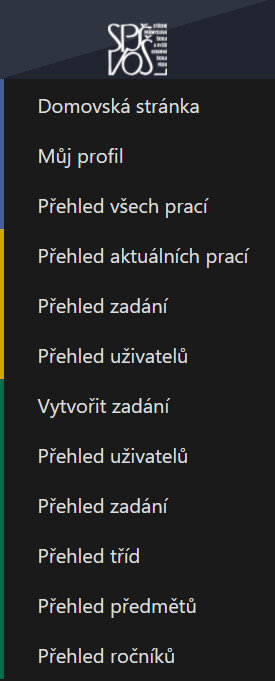
\includegraphics[scale=0.7]{Menu}
		\caption{Uživatelské menu se všema stránkama.}
		\label{Menu}
	\end{figure}
	\begin{listing}[H]
		\inputminted{html}{SourceCode/Views/Shared/_MenuPartial.html}
		\caption{View - \_MenuPartial.cshtml}
		\label{sharedmenupartial}
	\end{listing}

	\section{Controller}
	Poslední položkou v MVC vzoru je controller. Každá role (kromě vedení, to má stejná práva jako administrator) bude mít vlastní controller. V projektu mám celkem 4 role, jejich bližší popis je v kategorii \ref{Autorizace}\nameref{Autorizace}, to znamená, že zde budou 3 controllery pro~role a~k tomu 1 controller pro home adresář, kde je Domovská stránka (\viz{Controllers}).\par
	Protože každá role má mít vlastní controller, musel jsem nějaký způsobem ošetřit, aby uživatel např. s rolí studenta nemohl načíst view z controlleru pro administratora. Uživatele je tedy potřeba autorizovat\footnote{Autorizace je proces získávání souhlasu s provedením nějaké operace, povolení přístupu někam, k~někomu nebo něčemu.\cite{Autorizace}} k přístupu do controlleru. Pro tuto akci postačí napsat nad třídu kód viz zdrojový kód \ref{Autorize}.
	\begin{listing}[H]
		\inputminted{csharp}{SourceCode/Controllers/Autorize.cs}
		\caption{Controller - Autorizace}
		\label{Autorize}
	\end{listing}
	\begin{figure}[H]
		\centering
		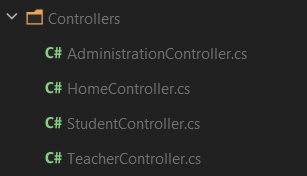
\includegraphics[scale=1]{Contollers}
		\caption{Složka Controllers}
		\label{Controllers}
	\end{figure}
	Jak již bylo zmíněno v teorii (viz kategorie \ref{Controller_teorie}\nameref{Controller_teorie}), controller pracuje s tzv. Action Method. V celé aplikaci mi postačí pouze 4 varianty Action Method, ve kterých se budou pouze měnit data. Ty varianty jsou:
	\begin{itemize}
		\item Zobrazit seznam entit
		\item Zobrazit detail položky
		\item Editovat položku
		\item Smazat položku
	\end{itemize}\par
	Před tím, než začnu popisovat jendotlivé varianty Action Method vypíši zde pro lepší přehlednost a srozumitelnost seznam využívaných metod a jejich výstup:
	\begin{itemize}
		\item NotFound() - NotFoundResult, který vrátí chybovou hlášku Error 404, stránka nenalezena.
		\item View() - Vytvoří objekt ViewResult, který vykreslí view na výstup.
	\end{itemize}
	A zde metody, které se využívají pro práci s entitami v Entity Framework:
	\begin{itemize}
		\item .Include() - Načte i související data. Např. K tabulce uživatelů načte i tabulku tříd.
		\item .AsNoTracking() - Entity Framework načte entity a již je dále nesleduje ani neukládá.
		\item .FirstOrDefaultAsync() - Asynchronně vrátí první prvek sekvence nebo výchozí hodnotu, pokud sekvence neobsahuje žádné prvky.
		\item .FindAsync() - Asynchronně nalezne entitu s danými hodnotami primárního klíče, pokud ji nalezne, vrátí ji okamžitě. V opačném případě vrací null\footnote{Označení pro žádnou hodnotu.}.
		\item .OrderBy() - Seřadí prvky v kolekci na základě zadaných polí ve vzestupném pořadí. Např. Na základě příjmení.
		\item .Where() - Načte pouze data, která splňují nějakou podmínku. Např. Načte pouze práce, kde je ID uživatele rovno přihlášenému uživateli.
	\end{itemize}

	\subsection{Seznam entit} \label{Seznam_entit}
	Jednou ze základních funkcí, kterou by měla tato webová aplikace disponovat je výpis seznamu entit (viz zdrojový kód \ref{ListOfEntit}). Pro to, abychom mohli entity vypsat, je potřeba je nejprve uložit do implicitně typované lokální proměnné var\footnote{Typ instance je odvozen z prvku zadaného v inicializátoru. To znamená, že kompilátor určí a přiřadí nejvhodnější typ proměnné.}. Do této vytvořené proměnné přiřadíme \_Contex.Users, což je metoda v AuthDBContext.cs. Právě tato třída je zodopovědná za interakci s databází. Poté pomocí .OrderBy(u => u.LastName) určím, že~chci řadit vzestupně podle proměné LastName, tedy příjmení. Protože s entitami již dále nepotřebuji pracovat, zakáži trasování pomocí .AsNoTracking().\par
	Takto jsem nadefinoval proměnou var users, kterou nyní stačí pouze uložit do List<T>\footnote{List (česky seznam) se řadí do kolekci, které umožňují prvky za běhu programu přidávat a mazat.}, a protože Task<IActionResul> požaduje asynchronní výstup, přidám k .ToList() klíčové slovíčko Async.\par
	Ná výstup se nám tedy vráti seznam uživatelů seřazený vzestupně podle příjmení, s~kterým dále pracuji ve view pomocí foreach().
	\begin{listing}[H]
		\inputminted{csharp}{SourceCode/Controllers/ListOfEntit.cs}
		\caption{Controller - Seznam entit}
		\label{ListOfEntit}
	\end{listing}

	\subsection{Detail} \label{Deail}
	Pokud chceme zobrazit detail některé entity, např. uživatele (viz zdrojový kód \ref{Detail}), potřebejeme nějakým jednoznačným způsobem definovat, o jakou entitu se jedná. Jedním z takových způsobů může být třeba primární klíč\footnote{Jednoznačná identifikace entity v rámci databáze.}. A nyní, jakým způsobem ji předat do~controlleru, aby s ní mohl pracovat? Přesně k tomu se využívají parametry v url\footnote{Uniform Resource Locator, neboli webová adresa.} adrese. Jak je vidět ve zdrojovék kódu\ref{Detail}, metoda UserOverview přebírá nějaký parametr, který nazýváme id a má datový typ string. Výsledná url může tedy vypadat například takto: \\
	https://localhost:5001/Administration/UserOverview/f0a5d163-b81c-41d1-a488-89\\753377fd1c\\
	Jako první se zde nachází protokol (https), po něm následuje doména (localhost:5001\footnote{Aplikace momentálně funguje na mém počítači, proto je doména localhost.}), a za doménou se vypíše jméno controlleru, ve kterém se nachází naše požadovaná stránka UserOverview. url zakončuje řetězec náhodných znaků, a to je právě id uživatele, tedy náš parametr.\par
	Tímto způsobem jsem tedy vyřešil identifikaci entity, které detail požadujeme zobrazit. A nyní zpět ke controlleru. Pokud controller dostane požadavek na detail entity, ověří nejprve, zda obdržel parametr id. Pokud ne, vyvolá metodu NotFound() a vrátí ji na výstup. V opačném případě se zahájí proces, která jsem podrobněji popisoval již v~předchozí kapitole (viz kapitola \ref{Seznam_entit}\nameref{Seznam_entit}).\par
	V detailu chci zobrazit základní údaje o uživateli a třídu, ve které se uživatel nachází. Controller prvně načte všechny uživatele z databáze, ale jak jsem zmínil, požaduji načtení i třídy. Protože u uživatele ukládám pouze ID třídy, ve které se nachází, musím přidružit i tabulku tříd. Toho docílím zavoláním metody .Include(c => c.Class). S daty nehodlám po načtení dále pracovat, proto mohu zakázat trasování.\par
	Úkolem metody FirstOrDefaultAsync(u => u.Id == id) je procházet entity, dokud nenajde první, jejíž Id je shodné s parametrem id. Pokud takovou entitu najde, vrací ji~na~výstup. Pokud takovou entitu nenajde, vrací výchozí hodnotu, kterou je null.\par
	Poslední podmínka ošetřuje situaci, kdy je zadán parametr, ale žádná entita tomuto parametru neodpovída. Pokud tedy nenajdeme žádného uživatele, který by měl shodné Id s parametrem id, zavolá se metoda NotFound(), která se vrátí na výstup.
	\begin{listing}[H]
		\inputminted{csharp}{SourceCode/Controllers/Detail.cs}
		\caption{Controller - Detail}
		\label{Detail}
	\end{listing}

	\subsection{Editace}
	Třetí typ stránky je určená k editaci. Pro to, abychom mohli entity upravovat, potřebujeme využít dvě metody. První metoda (viz zdrojový kód \ref{Edit}) má za úkol načíst data o~entitě z databáze, druhá následně upravená data odeslat zpět do~databáze.\par
	Při načítání dat je princip stejný, jak u načítání detailu (viz kapitola \ref{Detail}\nameref{Detail}), opět přebíráme parametr z url. Pokud se tam nachází, hledáme pomocí metody FindAsync(id) idetitu, jejiž primární klíč je shodný s naším parametrem. Pokud se parametr nenalezne, vyvolá se metoda NotFound(), která vrátí na výstup chybovou hlášku. Následně ověříme, zda se nějaká entita nalezla, pokud ne, controller vrací chybovou hlášku.\par
	Protože se jedná o editaci, potřebuji načíst seznam všech tříd tak, abych mohl případně změnit uživateli třídu. Z toho důvodu jsem si vytvořil metodu s názvem PopulateClassesWithIdDropDownList() (viz zdrojový kód \ref{DropDownList}), která ma za úkol načíst všechny entity z~tabulky tříd, a jejich Id a název vložit do drop-down menu.
	\begin{listing}[H]
	\inputminted{csharp}{SourceCode/Controllers/Edit.cs}
	\caption{Controller - Editace, načtení entit)}
	\label{Edit}
	\end{listing}
	Máme načtenou stránku s entitami, provedeme změny a chceme je odeslat zpět do databáze. V tuto chvíli využijeme druhou metodu (viz zdrojový kód \ref{Edit_Post}), která má provést změny v databázi. Protože se dvě metody nemohou nazývat stejným jménem, musím této metodě přidělit pomocí atributu tzv. ActionName, které následně volám z view. V~atributech mimo jiné nastavím i dotazovací metodu (tedy HttpPost) a ValidateAntiForgeryToken. ValidateAntiForgeryToken je ochrana proti padělání požadavků mezi weby. MVC zapíše jedinečnou hodnotu do cookies a tatéž hodnota se zapíše i do formuláře. Před odesláním formuláře se tyto hodnoty porovnají a pokud jsou různé, formulář se~neodešle.\par
	Controller zkontroluje parametr a pokud nenalezl chybu, načte první entitu, jejiž Id je shodné s parametrem, předaným v url. Následuje metoda TryUpdateModel, ta aktualizuje zadanou instanci modelu pomocí hodnot v paramteru (FirstName, LastName, atd.). Metodu zahrneme do podmínky. Pokud je podmínka splněna (nenastane chyba), asynchronně uloží všechny změny provedené v tomto kontextu a uloží je do databáze. Poté se přesměruje na stránku UsersOverview. Pokud nastane chyba (podmínka není splněna), vyvolá se větev catch, která vrátí chybovou hlášku.
	\begin{listing}[H]
		\inputminted{csharp}{SourceCode/Controllers/Edit_Post.cs}
		\caption{Controller - Editace, odeslání změn)}
		\label{Edit_Post}
	\end{listing}

	\subsection{Smazání}
	Posledním typem, který v práci využívám je smazání. Entity, které mají relaci s~některou jinou etitou nelze smazat.\par
	Podobně, jak tomu bylo u editace a vytvoření, i zde využívám 2 metody. První, která načítá stránku s možností potvrdit smazání nebo ho zrušit. Druhá, která provede samotné smazání entity.\par
	Pokud uživatel v seznamu entity vybere možnost smazat entitu, aplikace vyšle požadavek GET a načte view UserDelete (viz zdorojový kód \ref{Delete}). Na této stránce má uživatel možnost potvrdit smazání entity, nebo ho zrušit. Pokud se rozhodne pro smazání, vytvoří se požadavek POST, který zavolá metodu HttpPost UserDelete (viz zdorojový kód \ref{Delete_Post}), která smazání entity provede. V HttpPost UserDelete se nachází blok try-catch, který bude kontrolovat, zda nedošlo při aktualizaci databáze k chybě. Pokud k chybě dojde, metoda HttpPost UserDelete zavolá metodu HttpGet UserDelete a předá ji parametr, který indukuje, že při aktualizaci databáze došlo k chybě (\viz{DeleteUser_URL}).\par
	Metoda HttpGet UserDelete poté opět zobrazí potvrzovací stránku, společně s chybovou zprávou. Uživatel poté může požadavek opakovat, nebo ho zrušit.\par
	Parametr saveChangesError je při prvním volání metody HttpGet UserDelete false, to znamená, že tato metoda není volaná z důvodu chyby a nevypisuje tedy chybovou zprávu. Pokud ale tuto HttpGet UserDelete metodu volá metoda HttpPost UserDelete~v návaznosti na chybu při aktualizaci databáze, nastaví se saveChangesError na true a~proto se chybová zpráva vykreslí na stránce (\viz{DeleteUser_ErrorMessage}).
	\begin{figure}[h!]
		
\includegraphics[width=\textwidth]{DeleteUser_lista}
		\caption{Url při chybě aktualizace databáze.}
		\label{DeleteUser_URL}
	\end{figure}
	\begin{listing}[H]
		\inputminted{csharp}{SourceCode/Controllers/Delete.cs}
		\caption{Controller - HttpGet UserDelete}
		\label{Delete}
	\end{listing}
	\begin{figure}[h!]
		\centering
		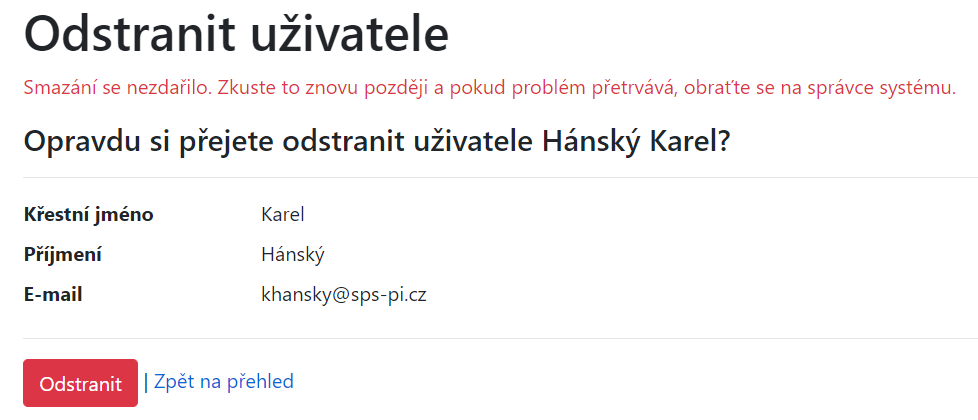
\includegraphics[scale=0.5]{DeleteUser}
		\caption{Chybová zpráva při chybě aktualizace databáze.}
		\label{DeleteUser_ErrorMessage}
	\end{figure}
	\begin{listing}[H]
		\inputminted{csharp}{SourceCode/Controllers/Delete_Post.cs}
		\caption{Controller - HttpPost UserDelete}
		\label{Delete_Post}
	\end{listing}
	
	
	\chapter{Přihlašování a registrace}
	Pro přihlašování a registraci uživatelů jsem využil APS.NET Core Identity. ASP.NET Core Identity je rozhraní API, které podporuje funkci přihlášení uživatelského rozhraní, spravuje uživatele, hesla, data profilu, role, deklarace identity, tokeny, potvrzení e-mailu a další \cite{ASP.NET_Core_Identity}.\par

	\section{Přihlášení}
	Přihlašovací formulář (\viz{PrihlasovaciFormular}) se zobrazí, pokud:
	\begin{itemize}
		\item Uživatel vybere možnost přihlásti se.
		\item Uživatel se pokusí zobrazit stránku, ke které nemá opravnění, nebo když ho aplikace nebyla schopna ověřit.
	\end{itemize}
	Při odeslání přihlašovacího formuláře se zavolá metoda OnPostAsync. V této metodě se volá objekt \_signInManager, který provede operaci PasswordSignInAsync. Dojde k~ověření uživatelského jména/e-mailu a hesla. Mimo jiné se zkontroluje, zda není zaškrtnuta možnost RememberMe, tedy pamatovat si přihlášení. Pokud je uživatel úspěšně ověřen, provede se autentizace uživatele, v opačném případě se vrátí chybová zpráva.\par
	Jestliže je zaškrtnuta možnost RememberMe, uloží se informace o identitě uživatele do~cookie. Pokud se uživatel odhlásí, zavolá se metoda LogoutModel.OnPost a v ní se provede operace SignOutAsync, která vymaže deklarace identity uživatele uložené v cookie.

	\section{Registrace}
	Když se chce uživatel registrovat, vyplní formulář na stránce Register (\viz{RegistracniFormular}) a odešle ho. Odeslání formuláře vyvolá metodu RegisterModel.OnPostAsync. Uživatel je~následně vytvořen pomocí objektu \_userManager, ve kterém se provede operace CreateAsync. CreateAsync vytvoří uživatele s parametry user a password (převede se na hash\footnote{Hašovací funkce je matematická funkce pro převod vstupních dat do malého čísla.\cite{Hash}} a následně uloží).\par
	Ve třídě IdentityHostingStartup.cs lze nastavit v services.AddDefaultIdentity<PPSPSUser> (viz zdrojový kód \ref{AddDefaultIdentity}), jaké požadavky musí splňovat heslo, aby bylo validní. Může se jednat například o povinnosti využít velká písmena, nealfanumerické znaky, atd. Lze nastavit i povinnost mít ověřený účet, jinak se uživatel nemůže přihlásit, dokud tak neučinní.

	\begin{figure}[H]
     \centering
     \begin{subfigure}[H]{0.45\textwidth}
         \centering
         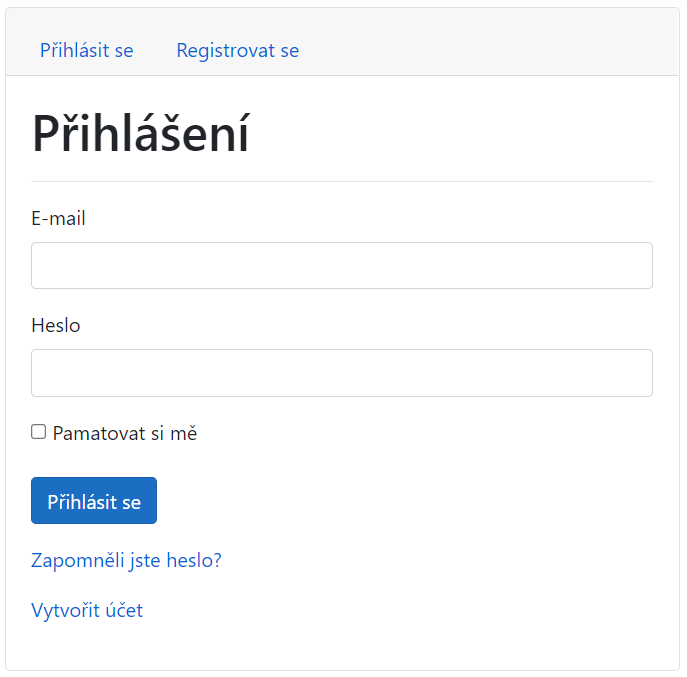
\includegraphics[width=\textwidth]{PrihlasovaciFormular}
         \caption{Přihlášení - Přihlašovací formulář}
         \label{PrihlasovaciFormular}
     \end{subfigure}
	 \hfill
     \begin{subfigure}[H]{0.45\textwidth}
         \centering
         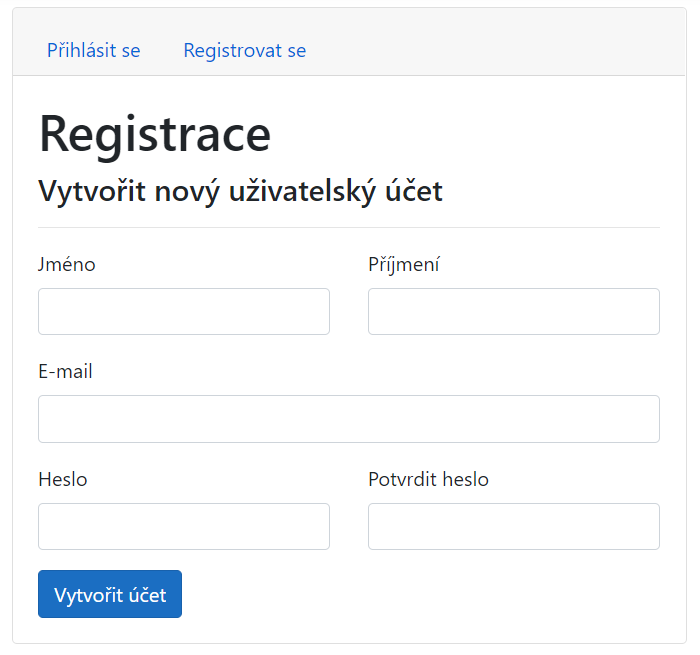
\includegraphics[width=\textwidth]{RegistracniFormular}
         \caption{Registrace - Registrační formulář}
         \label{RegistracniFormular}
     \end{subfigure}
        \caption{Formuláře pro přihlašování a registraci}
        \label{PrihlasovaniRegistrace}
\end{figure}
	\begin{listing}[H]
	\inputminted{csharp}{SourceCode/AddDefaultIdentity.cs}
	\caption{Registrace - services.AddDefaultIdentity<PPSPSUser>)}
	\label{AddDefaultIdentity}
	\end{listing}

	\chapter{Autorizace} \label{Autorizace}
	Autorizace se týká procesu, který určuje, co může uživatel dělat. Pro nastavení rolí využívám ASP.NET Core Authorization, ten poskytuje jednoduchou, deklarativní roli a~bohatý model založený na zásadách \cite{ASP.NET_Core_Autorizace}.

	\section{Student}
	První rolí je Student. Uživatelé s touto rolí mají možnost číst seznam aktuálních prací a k pracím se zapsat. Do zapsaných prací může student odevzdávat své řešení.\par
	Při registraci se uživatel automaticky přiřadí do této role. Děje se tak při procesu registrace, kde vyvolám objekt \_userManager s operaci AddToRoleAsync (viz zdrojový kód \ref{AddToRole}) a ta přidá uživatele do role z parametru.

	\begin{listing}[H]
		\inputminted{csharp}{SourceCode/AddToRole.cs}
		\caption{Student - Přířazení uživatele do role.}
		\label{AddToRole}
	\end{listing}

	\section{Učitel}
	Tato role má oprávnění vytvářet, editovat a mazat zadání a kontrolovat řešení, která odevzdají žáci. Zároveň má možnost zobrazit profil všech uživatelů a upravit ho. Uživatel musí být do této role přidán administratorem.
	\section{Administrator}
	Role administratora má všechny oprávnění pro správu webové aplikace. Je konstruována tak, aby pokud možno nemusel nikdo zasahovat přímo do databáze. To znamená, že~všechny akce s databází je možné provádět z uživatelského rozhraní.\par
	Administrator může vytvářet, upravovat nebo mazat předměty, třídy, ročníky, skupiny a samotná zadání.
	\section{Vedení školy}
	Poslední rolí je Vedení školy. Vzhledem k tomu, že uživatelé s touto rolí mají mít přehled o všech zadáních, třídách, uživatelích, atd. mají stejná opravnění jako administrator. Jediná věc, která tuto roli odlišuje od role Administrator je název. Důvodem je, aby bylo jasné, zda je uživatel administratorem webové aplikace, nebo členem vedení školy.

	\chapter{Databáze} \label{Databaze}
	\section{Propojení aplikace a databáze}
	Aby bylo možné propojit databázi s webovou aplikací, musím stáhnout package, který mi to dovolí. V této webové aplikaci využívám MySQL databázi, proto jsem si stáhl balíček MySql.Data.EntityFrameworkCore. To provedu přes NuGet Package Manager.\par
	V IdentityHostingStartup.cs je potřeba do metody Configure definovat DbContext, databázi, kterou využívám a connection string (v mém případě jen proměnou AuthDBContextConnection, ve které je connection string uložen) (viz zdrojový kód \ref{Databaze_Configure}).\par
	V appsettings.json následně vytvořím ConnectionString (viz zdrojový kód \ref{ConnectionString}). Protože databáze momentálně fungu na localhostu, má IP adresu 127.0.0.1. Poté určím, jaké schéma chci načíst a pod jakou identitou se chci přihlásit.

	\begin{listing}[H]
		\inputminted{csharp}{SourceCode/Databaze/Databaze.cs}
		\caption{Databáze - Services Configure}
		\label{Databaze_Configure}
	\end{listing}

	\begin{listing}[H]
		\inputminted{json}{SourceCode/Databaze/ConnectionString.json}
		\caption{Databáze - ConnectionString}
		\label{ConnectionString}
	\end{listing}

	\section{Návrh databáze}
	Celou databázi, kterou v aplikaci používám je vidět na obrázku \ref{NavrhDatabaze}. V následujících podkapitolách nastíním, co je úkolem jaké tabulky.\par
	Tabulky, které začínají předponou aspnet... byly vygenerovány pomocí ASP.NET Core.
	\begin{figure}[h!]
		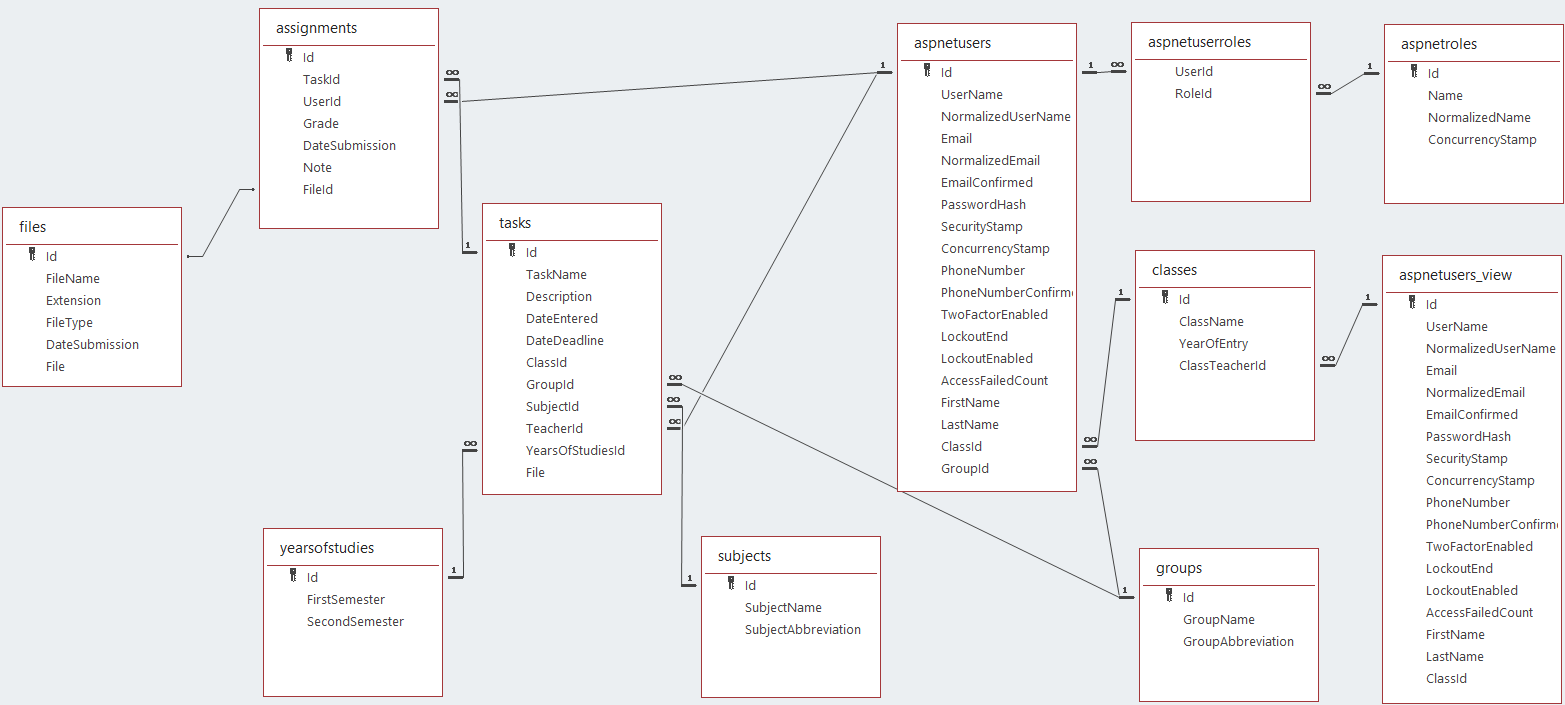
\includegraphics[width=\textwidth]{Databaze}
		\caption{Návrh databáze.}
		\label{NavrhDatabaze}
	\end{figure}

	\subsection{Aspnet tabulky}
	\begin{itemize}
		\item \textbf{Aspnetusers} - Obsahuje v sobě záznamy, které webová apolikace potřebuje pro~ověření Identity. Do tabulky jsem přidával pouze křestní jméno, příjmení, třídu a~skupinu. Jejím úkolem je identifikovat uživatele.
		\item \textbf{Aspnetroles} - Tabulka rolí.
		\item \textbf{Aspnetuserroles} - Tabulka propojující uživatele s rolemi.
	\end{itemize}

	\subsection{Vlastní tabulky}
	\begin{itemize}
		\item \textbf{Task} - Tabulka obsahující zadání prací. Pokud učitel vytvoří zadání, uloží ho právě do této tabulky.
		\item \textbf{Assignments} - Tabulka propojující uživatele, zadání, a soubor.
		\item \textbf{Classes} - Tabulka tříd.
		\item \textbf{Groups} - Tabulka skupin.
		\item \textbf{Subject} - Tabulka předmětů.
		\item \textbf{YearsOfStudies} - Tabulka ročníků. Ukládá ročník studia (např. 2020/2021).
		\item \textbf{Files} - Tabulka souborů.
	\end{itemize}

	\chapter{Závěr}
	Cílem této maturitní práce bylo vytvořit takovou webovou aplikaci, která umožní efektivní správu povinných prací, které žák zpracoval za celou dobu studia. V práci se nachází 3 základní role (student, učitel, administrátor), a 1 pro vedení školy.\par
	Student má možnost si procházet práce určené pro jeho třídu a popřípadě i skupinu. K~práci se následně může zapsat, čím dá najevo, že hodlá práci zpracovat a přidá se mu tedy i~do seznamu jeho prací. Dokud nebude práce hodnocena, má student možnost aktualizovat odevzdanou práci, datum se ale vždy aktualizuje na den poslední úpravy.\par
	Učitel má možnost vytvářet zadání, aktivní v určitém časovém intervalu. Zadání může specifikovat na třídu a nebo i na skupinu ve tříde.	Nabízí se mu i možnost procházet všechna svá zadání a v přehledné tabulce si zobrazit všechny studenty, kteří na vybrané práci pracovali. Do aplikace je přidána i možnost hodnocení.\par
	Administrátor má možnost z přívětivého uživatelského rozhraní spravovat běh webové aplikace. Má možnost přidávat jak předměty, skupiny a ročníky studia, tak i třídy a~studenty do nich. Podobně jako Vedení školy má možnost nahlížet do jednotlivých prací a~mít tak přehled o plnění a četnosti povinných prací.\par
	Tato webová aplikace je celá navržena a vytvořena na moderním frameworku ASP.NET Core, který ji dovoluje implementovat na platformách Windows, Linux i macOS. Zároveň dosahuje vysokých výkonů a disponuje kvalitním zabezpečením.\par
	Práci jsem prozatím nepropojoval se školním LDAP serverem, místo toho webová aplikace využívá ASP.NET Core Identity. Ta poskytuje bezpečné přihlašování a uchovávání osobních údajů. Volil jsem takto z důvodu testování, abych v této fázi nemusela být webová aplikace připojena do ostré databáze.\par
	Díky architektonickému vzoru MVC lze tuto aplikaci i nadále rozvíjet a doplňovat o~další funkce. Věřím, že tato webová aplikace nalezne svoje využití a bude prospěšná.

	\seznamObrazku

	\renewcommand\listoflistingscaption{Seznam zdrojových kódů}
	\listoflistings
	

	\bibliographystyle{czechiso}
	\bibliography{main}

	\prilohy{
		\chapter{Příloha}
		\begin{listing}[H] \inputminted{csharp}{SourceCode/PopulateDropDownList.cs}
		\caption{Drop-down list ze seznamu tříd}
		\label{DropDownList}
		\end{listing}
	}

\end{document}